% July 2015
% Autor: Mandy Vogel
% modelling

\documentclass[xcolor={table},handout]{beamer}
\usepackage{amssymb,amsmath}
%\documentclass[xcolor={table}]{beamer}
% \usetheme[backgroundimagefile=mathe]{diepen}
\usetheme{Singapore}
\useoutertheme{miniframes}

%\setbeamerfont{block title}{size=\small,series=\bfseries}
%\setbeamerfont{block body}{size=\footnotesize}

% \usecolortheme{beetle}
\usepackage{linkimage}

%\usepackage{handoutWithNotes}
%\pgfpagesuselayout{2 on 1}[a4paper,border shrink=5mm]
%\pgfpagesuselayout{3 on 1 with notes}[a4paper,border shrink=5mm]

\begin{document}

\title{Modelling}   
\author{Mandy Vogel} 
\date{\today}

\AtBeginSection{
  \begin{frame}<beamer>{Table of Contents}
    \tableofcontents[currentsection]
  \end{frame}}

\begin{frame}
\titlepage
\end{frame}

\begin{frame}{Table of Contents}
\frametitle{Table of Contents}\tableofcontents
\end{frame}

\section{Introduction}
\subsection{Choosing a Method}
\begin{frame}\frametitle{Choosing the appropriate method}
It is essential, therefore, that you can answer the following questions:
\begin{itemize}
\item Which of your variables is the response variable?
\item Which are the explanatory variables?
\item Are the explanatory variables continuous or categorical, or a mixture of both?
\item What kind of response variable do you have: is it a continuous measurement, a count, a proportion, a time at death, or a category?
\end{itemize}
%These simple keys will lead you to the appropriate statistical method:
%A data frame with 500 observations on the following 8 variables. 
%From: Michael Hills and Bianca De Stavola (2002). A Short Introduction
%     to Stata 8 for Biostatistics, Timberlake Consultants Ltd <URL:
%     http://www.timberlake.co.uk>
\end{frame}

\begin{frame}\frametitle{Choosing the appropriate method}
\begin{center}\small
    \rowcolors[]{1}{gray!10}{gray!30}
  \begin{tabular}{@{} >{\ttfamily}l l} 
    \rowcolor{gray!40}
Explanatory Variables are & \\
all  continuous                  & Regression                     \\ 
all categorical & Analysis of variance (ANOVA)   \\
both continuous and categorical & Analysis of covariance (ANCOVA)\\
  \end{tabular}
\end{center}
\end{frame}

\begin{frame}\frametitle{Choosing the appropriate method}
\begin{center}
    \rowcolors[]{1}{gray!10}{gray!30}
  \begin{tabular}{@{} >{\ttfamily}l l} 
    \rowcolor{gray!40}
Response Variables & \\
(a) Continuous   & Normal regression, ANOVA or ANCOVA\\
(b) Proportion   & Logistic regression               \\
(c) Count        & Log-linear models                 \\
(d) Binary       & Binary logistic analysis          \\
(e) Time at death& Survival analysis                 \\
  \end{tabular}
\end{center}
The best model is the model that produces the \textbf{least unexplained variation} (the minimal residual
deviance), subject to the constraint that \textbf{all the parameters} in the model \textbf{should be statistically
significant}.
\end{frame}

\begin{frame}\frametitle{Choosing the appropriate method}
It is very important to understand that there is not \textit{one} model; this is one of the common implicit errors involved in traditional regression and ANOVA, where the same models are used, often uncritically, over and over again. In most
circumstances, there will be a large number of different, more or less plausible models that
might be fitted to any given set of data. 

And of course: We are looking for the BEST.
\end{frame}

\begin{frame}\frametitle{Maximum Likelihood}
We define \emph{best} in terms of maximum likelihood.
\begin{itemize}
\item given the data,                                                                
\item and given our choice of model,                                                 
\item what values of the parameters of that model make the observed data most likely?
\end{itemize}
We judge the model on the basis how likely the data would be if the model were correct. 
\end{frame}

\begin{frame}\frametitle{Ockham's Razor}

For statistical modelling, the principle of
parsimony means that:
\begin{itemize}
\item models should have as few parameters as possible;
\item linear models should be preferred to non-linear models;
\item experiments relying on few assumptions should be preferred to those relying on many;
\item models should be pared down until they are minimal adequate;
\item simple explanations should be preferred to complex explanations.
\end{itemize}
\end{frame}

\subsection{Types of Models}

\begin{frame}\frametitle{The Null model}
\begin{columns}
\begin{column}{0.6\textwidth}
\linkimage{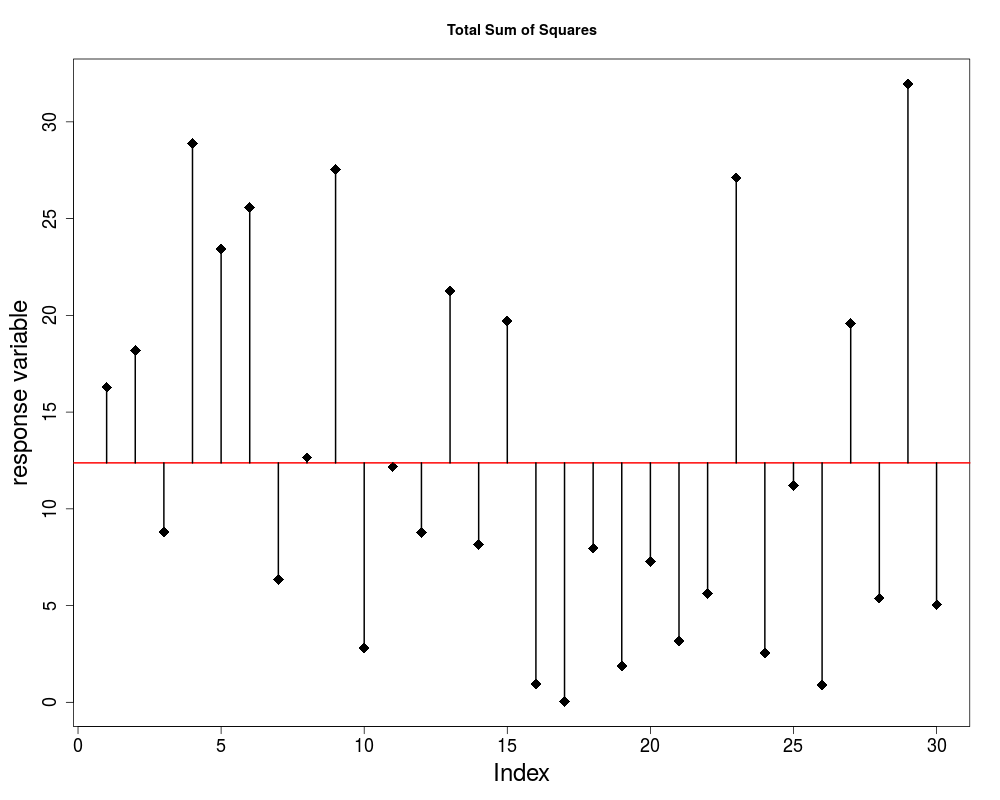
\includegraphics[width=6.5cm]{nullmodel.png}}{nullmodel.png}
\end{column}
\begin{column}{0.4\textwidth}
\begin{itemize}
\item Just one parameter, the overall mean $\bar{y}$
\item Fit: none; $SSE = SSY$
\item Degrees of freedom: $n-1$
\item Explanatory power of the model: none
\end{itemize}
\end{column}
\end{columns}
\end{frame}

\begin{frame}\frametitle{Adding Information}
\begin{columns}
\begin{column}{0.6\textwidth}
\linkimage{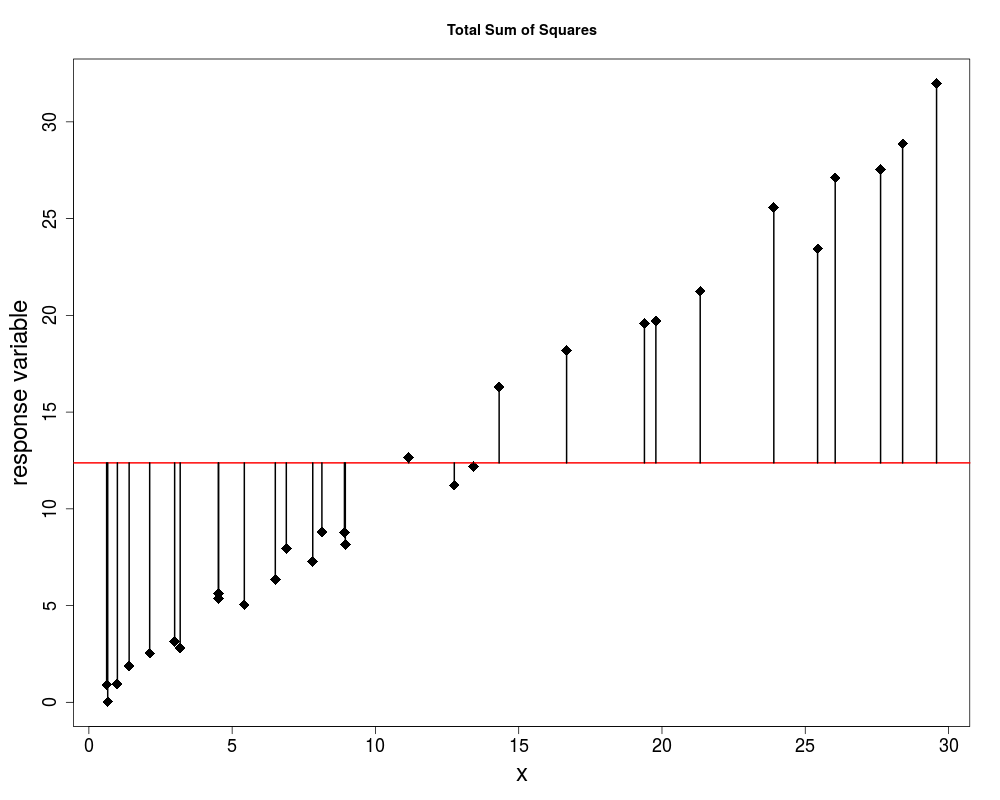
\includegraphics[width=6.5cm]{minimalmodel.png}}{minimalmodel.png}
\end{column}
\begin{column}{0.4\textwidth}
\begin{itemize}
\item model with $0 \le p' \le p$ parameters
\item Fit: less than the maximal model, but not significantly so
\item Degrees of freedom: $n-p'-1$
\item Explanatory power of the model: $r^2 = \frac{SSR}{SSY}$    
\end{itemize}
\end{column}
\end{columns}
\end{frame}

\begin{frame}\frametitle{Adding Information}
\begin{columns}
\begin{column}{0.6\textwidth}
\linkimage{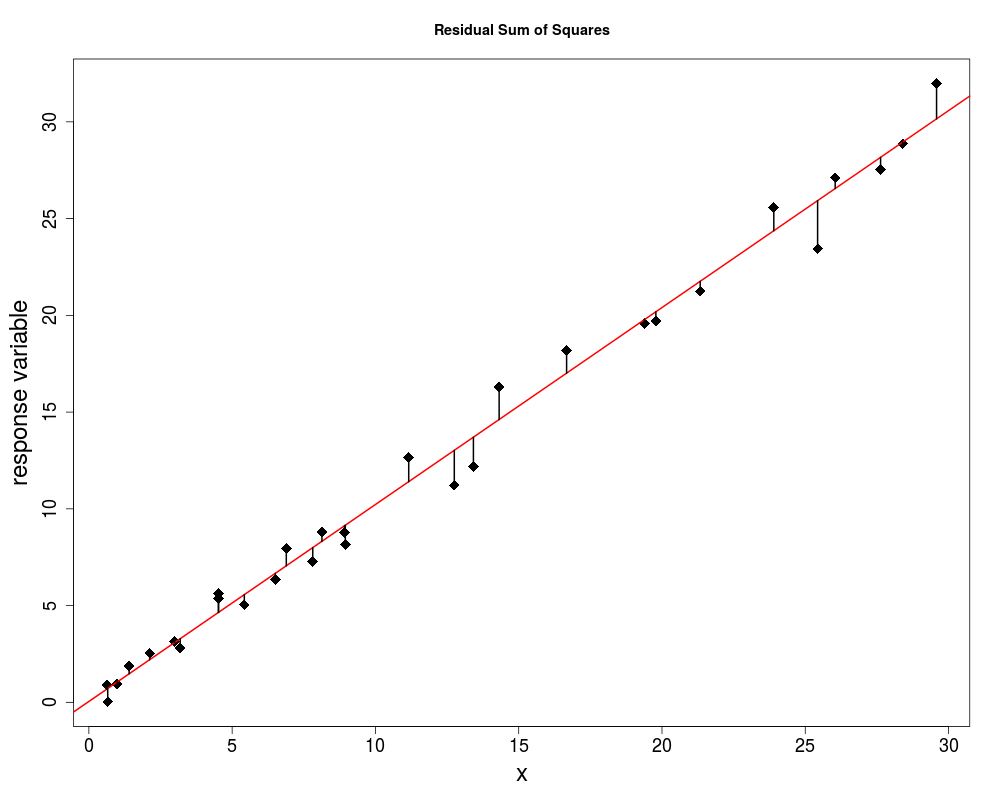
\includegraphics[width=6.5cm]{minimalmodel2.png}}{minimalmodel2.png}
\end{column}
\begin{column}{0.4\textwidth}
\begin{itemize}
\item model with $0 \le p' \le p$ parameters
\item Fit: less than the maximal model, but not significantly so
\item Degrees of freedom: $n-p'-1$
\item Explanatory power of the model: $r^2 = \frac{SSR}{SSY}$    
\end{itemize}
\end{column}
\end{columns}
\end{frame}

%% \begin{frame}\frametitle{Saturated/Maximal Model}
%% \begin{columns}[t]
%% \begin{column}{0.5\textwidth}
%% saturated model
%% \begin{itemize}
%% \item One parameter for every data point
%% \item Fit: perfect
%% \item Degrees of freedom: none
%% \item Explanatory power of the model: none
%% \end{itemize}
%% \end{column}
%% \begin{column}{0.5\textwidth}
%% maximal model
%% \begin{itemize}
%% \item Contains all $p$ factors, interactions and covariates that
%% \item might be of any interest. Many of the model’s terms are likely to be insignificant
%% \item Degrees of freedom: $n-p-1$
%% \item Explanatory power of the model: it depends
%% \end{itemize}
%% \end{column}
%% \end{columns}
%% \end{frame}

%% \begin{frame}\frametitle{How to choose...}
%% \begin{itemize}
%% \item models are representations of reality that should be both accurate and convenient
%% \item it is impossible to maximize a model’s realism, generality and holism simultaneously
%% \item the principle of parsimony is a vital tool in helping to choose one model over another
%% \item only include an explanatory variable in a model if it significantly improved the fit of the model
%% \item the fact that we went to the trouble of measuring something does not mean we have to have it in our model
%% \end{itemize}
%% \end{frame}


\section{Modelling in R}
\subsection{Model Formulae in R}
\begin{frame}\frametitle{General Formula Syntax}
\begin{center}
\large 
\textbf{response variable $\sim$ explanatory variable(s)}

\vspace*{1.5cm}

one can read the tilde symbol as \emph{is modelled as a function of}
\end{center}
\end{frame}

\begin{frame}[fragile]\frametitle{Simple Linear Regression}
\begin{center}
\large 
\begin{math}\mbox{lm}(y\sim x)\end{math}
\end{center}
\begin{exampleblock}{Output}
\begin{semiverbatim}
Call:
lm(formula = y ~ x, data = df)

Coefficients:
(Intercept)            x  
    -0.1253       1.0207  
\end{semiverbatim}
\end{exampleblock}
\end{frame}

\begin{frame}[fragile]\frametitle{Simple Linear Regression}
The model contains much more information. We can access them if we assign it to a variable.
\begin{exampleblock}{Input}
\begin{semiverbatim}
> m <- lm(y~x,data=df)
> summary(m)
\end{semiverbatim}
\end{exampleblock}
\end{frame}

\begin{frame}[fragile]\frametitle{Simple Linear Regression}
\begin{exampleblock}{Output}\footnotesize
\begin{semiverbatim}
Call:
lm(formula = y ~ x, data = df)

Residuals:
     Min       1Q   Median       3Q      Max 
-1.30324 -0.59581  0.00489  0.57777  1.42182 

Coefficients:
            Estimate Std. Error t value Pr(>|t|)    
(Intercept)  -0.1253     0.3658  -0.343    0.735    
x             1.0207     0.0203  50.293   <2e-16 ***
---
Signif. codes:  0 ‘***’ 0.001 ‘**’ 0.01 ‘*’ 0.05 ‘.’ 0.1 ‘ ’ 1 

Residual standard error: 0.7412 on 28 degrees of freedom
Multiple R-squared: 0.9891,	Adjusted R-squared: 0.9887 
F-statistic:  2529 on 1 and 28 DF,  p-value: < 2.2e-16 
\end{semiverbatim}
\end{exampleblock}
\end{frame}

\begin{frame}[shrink=3,fragile]\frametitle{Simple Linear Regression}
With \texttt{aov(m)} you can fit an analysis of variance model for each stratum.
\begin{exampleblock}{Input}
\begin{semiverbatim}
> aov(m)
\end{semiverbatim}
\end{exampleblock}
\begin{exampleblock}{Output}\footnotesize
\begin{semiverbatim}
Call:
   aov(formula = m)

Terms:
                        x Residuals
Sum of Squares  1389.7606   15.3842
Deg. of Freedom         1        28

Residual standard error: 0.7412399 
Estimated effects may be unbalanced
\end{semiverbatim}
\end{exampleblock}
\end{frame}

\begin{frame}\frametitle{Notation}
\begin{center}
    \rowcolors[]{1}{gray!10}{gray!30}
  \begin{tabular}{@{} >{\ttfamily}l p{9cm}} 
    \rowcolor{gray!40}
symbol & meaning\\
$+$ & indicates inclusion of an explanatory variable in the model (not addition)\\
$-$ & indicates deletion of an explanatory variable from the model (not subtraction)\\
$*$ & indicates inclusion of explanatory variables and interactions (not multiplication)\\
$/$ & indicates nesting of explanatory variables in the model (not division)\\
$|$ & indicates conditioning (not ``or''), so that $y \sim x | z $ is read as $y$ as a function of $x$ given $z$.\\
\end{tabular}
\end{center}
$A:B$ means the two way interaction between $A$ and $B$ and $A:B:C:D$ means the four-way interaction between the four variables.
\end{frame}

\begin{frame}\frametitle{Notation 2}
A term of the form \texttt{A/x} where \texttt{A} is a factor, gives ``separate'' regression lines of type $1+x$ for different levels of \texttt{A}. In this case the intercept term is not needed (removed by \texttt{-1}).

Another important function term is the identity function \texttt{I(...)}. It is used to evaluate its argument with operators having their arithmetical meaning and returns the result. 
\end{frame}

\section{Examples}

\begin{frame}\frametitle{examples}
\begin{center}\footnotesize
    \rowcolors[]{1}{gray!10}{gray!30}
  \begin{tabular}{p{1.5cm} >{\ttfamily}p{2cm} p{6.2cm}} 
    \rowcolor{gray!40}
Model&Formula&Comments\\
Null&$y\sim 1$&is the intercept in regression models, but here it is the overall mean y\\
Regression&$y\sim x$ &x is a continuous explanatory variable\\
Regression through origin &$y \sim x-1$ & Do not fit an intercept\\
One-way ANOVA&$y \sim sex$ &sex is a two-level categorical variable\\
One-way ANOVA&$ y \sim sex-1$& as above, but do not fit an
                       intercept (gives two means
                      rather than a mean and a
                     difference)\\
Two-way ANOVA&$y \sim sex + genotype$&genotype is a three-level
                                catEegorical variable\\
Analysis of covariance&$y \sim x + sex$& A common slope for y against
                                  x but with two intercepts, one
                                 for each sex\\
Analysis of covariance&$y \sim x * sex$& Two slopes and two intercepts\\
\end{tabular}
\end{center}
\end{frame}

\begin{frame}\frametitle{examples}
\begin{center}\footnotesize
    \rowcolors[]{1}{gray!10}{gray!30}
  \begin{tabular}{p{1.5cm} >{\ttfamily}p{2cm} p{6.2cm}} 
    \rowcolor{gray!40}
Model&Formula&Comments\\
Multiple regression&$y\sim x + z$& Two continuous explanatory
                           variables, flat surface fit\\
Multiple regression&$y\sim x * z$& Fits an interaction term as well
                           (x + z + x:z)\\
Multiple regression &$y \sim x + I(x^2) + z + I(z^2)$& Fit a quadratic term for both x
                                               and z\\
Multiple regression&$y \sim poly(x,2) + z$& Fit a quadratic polynomial for x
                                      and linear z\\
Multiple regression&$y \sim (x + z + w)^2$& Fit three variables plus all their
                                     interactions up to two-way
\end{tabular}
\end{center}
\end{frame}




\appendix
\flushlinkimages

\end{document}

